\section{Digital-Analog-Umsetzung}\label{4}

Mithilfe des in [\ref{3}] beschriebenen Verfahrens wurde ein analoges Signal in eine digitale Form konvertiert. Von ebenso großer Bedeutung ist die Wandlung eines digitalen- in ein analoges Signal, beispielsweise im Anschluss an die Signalverarbeitung mithilfe eines DSP.

\subsection{Theorie}
Im Folgenden werden zunächst die Limitierungen eines Digital-Analog-Umsetzers (DA-Umsetzer) aufgeführt. Anschließend wird das theoretische Verfahren dieser Umsetzung beschrieben, wobei auch auf benötigte Filter eingegangen wird. Zuletzt folgen Abweichungen und Fehlerabschätzungen.

\subsubsection{Limitierungen eines DA-Umsetzers}
Einem DA-Wandler ist es in der Regel nicht möglich, ein digitales (diskretes) Signal in ein wertkontinuierliches analoges Signal zu überführen. Dabei schränkt die Quantisierungsstufe aus [\ref{3.1.5}] das Verfahren nicht ein. Wird das Abtasttheorem eingehalten, so ist es möglich, das Signal in dem zu Grunde liegenden System digital zu rekonstruieren und so eine beliebig genaue Auflösung zu erstellen.\\
Ein DA-Wandler besitzt jedoch nur $n$ verschiedene Stufen, die er darstellen kann. Somit kann selbst ein beliebig genau aufgelöstes Signal nicht wertkontinuierlich ausgegeben werden.\\
Es ergibt sich, dass ein DA-Wandler beliebig komplex werden kann, um die nötige Anzahl an Stufen darstellen zu können. Allerdings ist die Realisierung solch einer feinen Auslösung nicht immer möglich, da ab kleineren Dimensionen das natürlich existierende Rauschen überwiegen und die feineren Stufen überdecken wird.\\
Weiterhin schränkt die Schaltgeschwindigkeit des Wandlers die Ausgabefrequenz ein. Für jeden Datenpunkt muss dieser dem DA-Wandler in entsprechender Form übergeben werden. Dieser muss die Ausgangsspannung entsprechend dem Datum anpassen und ausgeben, ehe ein neues Datum angenommen werden kann.\\
DA-Wandler sind somit nicht in der Lage, Frequenz der Datenpunkte oder Auflösung des ausgegebenen Signals beliebig anzupassen, sondern sind durch physikalische- sowie durch Gatterlaufzeiten bestimmte Grenzen limitiert.

\subsubsection{Verfahren}
Die Theorie eines DA-Wandlers ist vergleichsweise simpel. Er besitzt $n$ Stufen, welche die maximale Ausgangsspannung meist linear unterteilen. Das eingehende Datum entscheidet darüber, welche dieser Stufen auf den Ausgang geschaltet wird.\\
Dieser Wert wird von einem nachfolgenden Eingangsregister gespeichert, bis ein neues Datum verarbeitet wurde. Das sich somit ergebende Bild ähnelt dem roten Signal aus [\ref{sah_signal}].

\begin{figure}[h!]
\centering
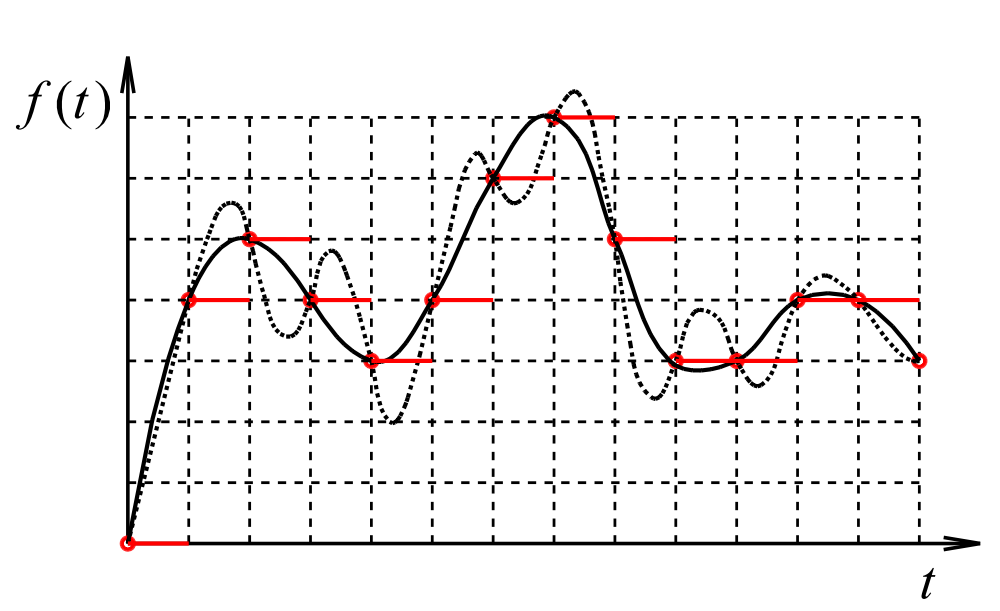
\includegraphics[scale=0.3]{images/dau_t.png}
\captionsource{Ausgabe eines DA-Umsetzers.}{\cite{dau_signal}}
\label{dau_signal}
\end{figure}

Das in [\ref{dau_signal}] rot gezeichnete Signal entspricht der idealen Ausgabe des Umsetzers. Das schwarz gestrichelte Signal beschreibt eine mögliche kontinuierliche Form des tatsächlichen Signals, welche höhere Frequenzanteile als die eigentliche bandbegrenzende Frequenz $f_{max}$ besitzt. Grund hierfür sind höhere Frequenzanteile, welche sich mit dem eigentlichen Signal überlagern. Durch das in [\ref{3.2.2}] beschriebene Spektrum des abgetasteten Signals wird ersichtlich, dass die Anteile höherer Frequenzen durch die $si$-Funktion schwächer gewichtet werden. Deshalb ist in [\ref{dau_signal}] der grobe Verlauf des Signals ersichtlich, während die höheren Frequenzen um dieses Signal herum oszillieren.\\

Zur Vermeidung dieser Überlagerung wird das entstehende Signal in der Regel mithilfe eines Anti-Aliasing-Filters behandelt. Dieser kann beispielsweise aus einem Tiefpassfilter mit Grenzfrequenz $f_G =\frac{f_A}{2}$ realisiert werden. In [\ref{2fsig}] wird ersichtlich, dass dies das Signal an dessen oberer Grenzfrequenz von den Kopien höheren Frequenzen isoliert. Wird eine Abtastfrequenz $$2f_{max} < f_A $$ gewählt, so kann die Grenzfrequenz des Filters ebenfalls angepasst werden. Entspricht diese exakt der halben Abtastfrequenz, so werden Anteile des eigentlichen Signals abgeschnitten, da ein reales Filter nicht ideal ist. Dies entspricht der Theorie aus [\ref{3.1.4}] sowie [\ref{3.2.2}].

\subsubsection{Abweichungen und Fehlerabschätzung}
\label{4.1.3}
Ein nicht vermeidbarer Fehler bei der DA-Wandlung ist der Quantisierungsfehler, welcher in [\ref{3.1.5}] vorgestellt wurde. Jeder Wert des originalen Signals hat eine Abweichung von maximal $\frac{\delta}{2}$, wobei $\delta$ die Quantisierungsstufe ist. Wird angenommen, dass das zu Beginn vorliegende analoge Signal im Wertebereich gleichverteilt ist, so ergibt sich der mittlere Quantisierungsfehler zu $$E_{mean} = \frac{\delta}{4}$$
Durch eine genauere Abtastung oder Rekonstruktion des digitalen Signals verbunden mit einer höheren Auflösung des DA-Umsetzers kann dieser Fehler reduziert werden.\\

\begin{figure}[h!]
\centering
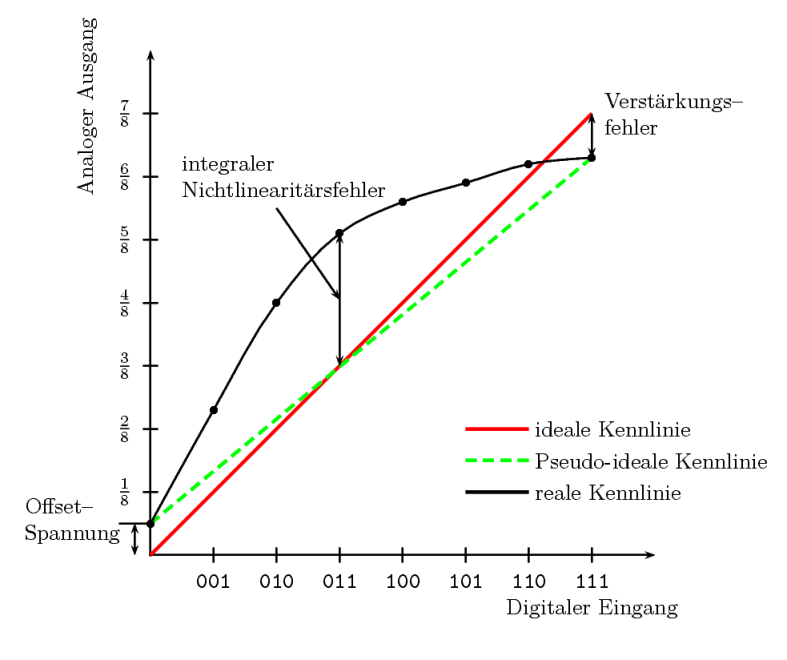
\includegraphics[scale=0.9]{images/dau_line.png}
\captionsource{Mögliche Fehler eines DA-Umsetzers.}{\cite{dau_line}}
\label{dau_line}
\end{figure}

[\ref{dau_line}] zeigt drei weitere mögliche Fehlerquellen auf. Zunächst kann ein Umsetzer eine Offset-Spannung besitzen. Dies bedeutet, dass ohne eingehendes Datum eine Grundspannung ausgegeben wird.\\
Der Verstärkungsfehler tritt ein, wenn die Ausgabe des Umsetzers mit einem Operationsverstärker (oder einem anderen Verstärker) verbunden wird. Ist die von diesem ausgehende Verstärkung falsch gewählt, so entspricht sie nicht der realen Steigung und führt zu weiteren Fehlern.\\
Zudem kann es zu Nichtlinearitäten kommen. Dies geschieht, wenn die Ausgangsspannung für einen steigenden digitalen Wert nicht in linearem Maß ansteigt. All diese Fehler treten in einer gewissen Intensität immer auf, können jedoch durch ein sorgsames Design des Systems minimiert werden.\\
Zuletzt kann es zu einer nicht stetigen Kennlinie kommen. Bei Verfahren, welche jedes eingehende Bit einzeln verarbeiten und das Ergebnis aufsummieren, ist es möglich, dass beispielsweise die Summe für das Eingangsdatum 01111111 größer als die für das Datum 10000000 ist, da bei dem ersten Datum sieben Werte addiert werden, was durch Ungenauigkeiten zu einer größeren Ausgangsspannung führen kann.

\subsection{Implementierung eines DAU}
Im Folgenden werden zwei einfache Verfahren vorgestellt, welche ein Digitales in ein analoges Signal überführen. Dabei wird besonderer Wert auf deren Vor- und Nachteile gelegt.


\subsubsection{Realisierung mithilfe eines Spannungsteilers}
\label{4.2.1}
\begin{figure}[h!]
\centering
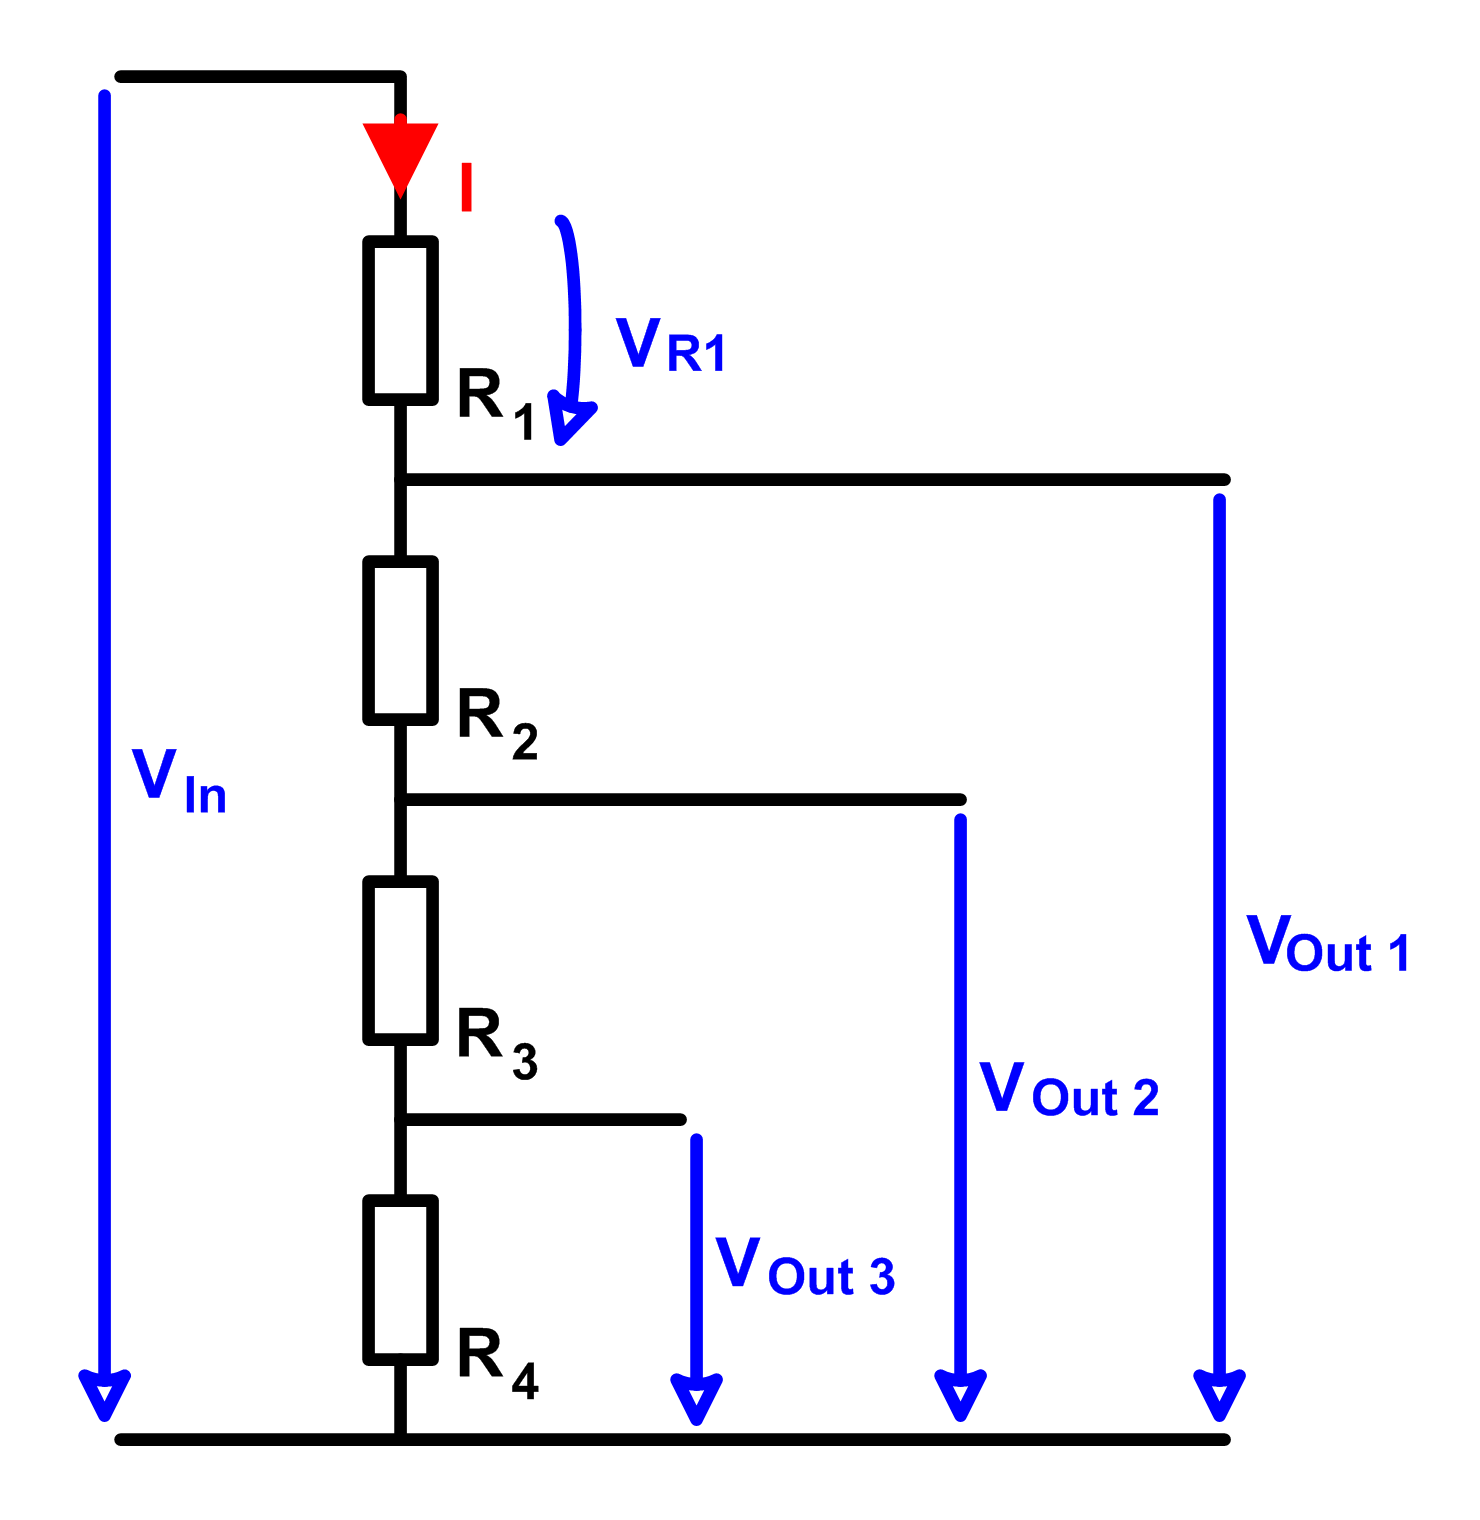
\includegraphics[scale=0.9]{images/spannteil.png}
\captionsource{Schematische Anordnung eines Spannungsteilers.}{\cite{spannteil}}
\label{spannteil}
\end{figure}

Zunächst wird eine konstante Versorgungsspannung $U_{in}$ an den Spannungsteiler angelegt, wobei $U_{in} = max(U_r)$ und $U_r$ die Sägezahnspannung aus [\ref{3.3.2}] ist. Die Anzahl der Widerstände entspricht der Anzahl an Quantisierungsstufen weniger Eins. Hierbei ist deren Widerstandswert irrelevant, lediglich müssen alle Widerstände den gleichen Wert besitzen. Anschließend liegt vor dem ersten Widerstand $U_{Out} = U_{in}$ an, nach dem letzten Widerstand $U_{Out} = 0$V. Nach dem $n$-ten von $k$ Widerständen ergibt sich die Ausgangsspannung $$U_{Out} = U_{in} \cdot \left( 1 - \frac{n}{k} \right)$$
Alle möglichen Ausgangsspannungen werden anschließend mit einen Multiplexer verbunden, welcher zusätzlich das aktuelle Datum des digitalen Signals erhält. Der entsprechende Spannungswert wird bis zur Ankunft des nächsten Datums als Ausgabe des DAU genutzt.\\
Diese Schaltung erfordert somit lediglich eine Reihe an Widerständen und einen Multiplexer mit entsprechend vielen Eingängen. Dies ist die simpelste Form der Realisierung eines DAU und bietet ein monotones Verhalten, verhindert also, dass der letzte in [\ref{4.1.3}] angesprochene Fehleraspekt auftreten kann.\\
Der Nachteil hier ist, dass die Anzahl an Widerständen linear mit der Anzahl an Quantisierungsstufen steigt. Für eine gewünschte Ausgabeauflösung von 10bit würden also 1023 Widerstände benötigt werden.

\subsubsection{Realisierung mithilfe eines R2R-Netzwerks}

\begin{figure}[h!]
\centering
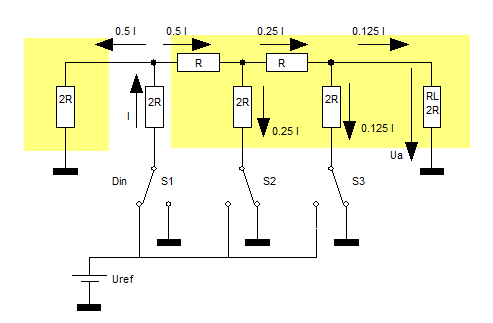
\includegraphics[scale=0.6]{images/r2r.png}
\captionsource{Schematische Anordnung eines R2R-Netzwerkes.}{\cite{r2r}}
\label{r2r}
\end{figure}

[\ref{r2r}] beschreibt den Aufbau eines R2R Netzwerkes. $U_{ref}$ bezeichnet die Versorgungsspannung, welche beliebig wählbar ist. Wie in [\ref{4.2.1}] ist auch hier der Wert von $R$ frei wählbar.\\
Für jedes Bit des digital vorliegenden Datums wird ein Schalter implementiert, welcher die Versorgungsspannung mit dem Netzwerk verbindet. Für den in [\ref{r2r}] linken Schalter 1 wird dessen Strom $I = \frac{U_{ref}}{3R}$ gleichmäßig nach links und rechts aufgeteilt, da beide Zweige einen identischen Gesamtwiderstand haben. Nach dem ersten Widerstand auf der rechten Seite geschieht eben dies ein weiteres Mal, sodass nun $\frac{I}{4}$ weiter nach rechts fließen. Nach einem weiteren Schritt erreicht $\frac{I}{8}$ den Ausgangswiderstand, wo die Spannung $$U_{out} = \frac{I}{8}\cdot 2 R = \frac{U_{ref}}{12}$$ anliegt. Für die Schalter 2 und 3 liegen die Spannungen $U_{out} = \frac{U_{ref}}{6}$ und $U_{out} = \frac{U_{ref}}{3}$ an, da deren Ströme eine- beziehungsweise zwei Halbierungen weniger durchlaufen.\\
Werden mehrere Schalter zugleich geschlossen, so führt die Überlagerung der Ströme auch zu einer Addition der einzelnen Teilspannungen, sodass diese beliebig kombiniert werden können. Findet anschließend eine Skalierung mithilfe beispielsweise eines Operationsverstärkers statt, so kann die Ausgangsspannung beliebig angepasst werden. Ein Faktor von $$\frac{max(U_r)}{U_{ref}} \cdot \frac{3}{2}$$ würde dazu führen, dass die Schalter S1, S2 und S3 die Gewichtung $\frac{max(U_r)}{8}$, $\frac{max(U_r)}{4}$ und $\frac{max(U_r)}{2}$ bekommen. Bei hinreichen vielen Schaltern würde diese Skalierung für eine maximale Spannung von $U_{out} \approx max(U_r)$ sorgen, wenn alle Schalter geschlossen sind.\\
Ein Nachteil dieser Schaltung ist die in [\ref{4.1.3}] erwähnte nicht garantierte Stetigkeit durch die Addition einzelner Teilströme. Jedoch ist die Anzahl an Bauteilen im Vergleich zu [\ref{4.2.1}] gering, sie beträgt etwa $$3 \cdot \lceil l_d (n) \rceil$$ für n Quantisierungsstufen.\\
Ein weiterer Vorteil ist die Geschwindigkeit der Schaltung. Durch die parallele Anordnung der einzelnen Schalter und deren unabhängiges Verhalten ist eine vergleichsweise hohe Frequenz realisierbar. Somit ist dieses Netzwerk in einer Vielzahl an Systemen zu finden.